\documentclass[a4paper]{scrreprt}
\usepackage[left=4cm,bottom=3cm,top=3cm,right=4cm,nohead,nofoot]{geometry}
\usepackage{import,graphicx,tabularx,listings,enumitem,subcaption}
\usepackage{xparse,multirow}
\usepackage{xcolor}
\usepackage{graphicx}
\usepackage{booktabs}
\usepackage{longtable}
\usepackage{float}  
\setlength{\textfloatsep}{16pt}
\renewcommand{\labelenumi}{\alph{enumi})}
\renewcommand{\labelenumii}{\arabic{enumii}) }

% Base info for header
\newcommand{\baseinfo}[5]{
  \begin{center}
    \begin{tabular}{p{15cm}r}
      \vspace{-4.5pt}{ \Large \bfseries #1} & \multirow{2}{*}{} \\[0.4cm]
      #2 & \\[0.5cm]
    \end{tabular}
  \end{center}
  \vspace{-18pt}\hrule\vspace{6pt}
  \begin{tabular}{ll}
    \textbf{Maxim Zilke} & #4\\
    \textbf{Group:2} & #5\\
  \end{tabular}
  \vspace{4pt}\hrule\vspace{2pt}
  \footnotesize \textbf{Software Testing} \hfil - \hfil Summer 2024 \hfil - \hfil #3 \hfil - \hfil Sibylle Schupp / Daniel Rashedi \hfil \\
}

\lstdefinestyle{pythongrey}{
    language=Python,
    basicstyle=\ttfamily\small,
    keywordstyle=\color{blue},
    commentstyle=\color{gray},
    stringstyle=\color{green!50!black},
    backgroundcolor=\color{gray!10},
    showstringspaces=false,
    breaklines=true,
    frame=single,
    framesep=3pt,
    tabsize=4,
    numbers=left,
    numberstyle=\tiny\color{gray},
    numbersep=8pt,
    captionpos=b
}

% Question and answer environments
\newcounter{question}
\NewDocumentEnvironment{question}{m o}{%
  \addtocounter{question}{1}%
  \paragraph{\textcolor{red}{Task~\arabic{question}} - #1\hfill\IfNoValueTF{#2}{}{[#2]}}
  \leavevmode\\%
}{%
  \vskip 1em%
}

\NewDocumentEnvironment{aiTask}{}{
  \paragraph{\textcolor{red}{AI Review Task}}
  \leavevmode\\
}{
  \vskip 1em
}

\NewDocumentEnvironment{answer}{}{%
  \vspace{6pt}
  \leavevmode\\
  \textit{Answer:}\\[-0.25cm]
  {\color{red}\rule{\textwidth}{0.4mm}}
}{%
  \leavevmode\\
  {\color{red}\rule{\textwidth}{0.4mm}}
}

% ======= STUDENTS: START EDITING BELOW THIS LINE =======
\newcommand{\projectinfo}[4]{\baseinfo{Project Task 04 - Submission Sheet}{#1}{#2}{#3}{#4}}
\newcommand{\name}{[Maxim Zilke, Yossef Al Buni]}
\newcommand{\group}{[Group 2]}

\begin{document}
\projectinfo{Software Testing - Logic Coverage\small}{\today}{\name}{\group}

\addtocounter{question}{3}

%%%%%%%%%%%%%%%%
%%% Phase 04 %%%
%%%%%%%%%%%%%%%%

\begin{question}{Logic Coverage}
  \begin{enumerate}[topsep=0pt, leftmargin=*]
    \item Pick a method of your given project which contains at least \textbf{2} predicates, with one of these predicates containing at least \textbf{3} clauses. If you cannot find a three-clause-predicate in your code, you can decide to take a nested structure of \textit{if-else} and/or nested \textit{while} expressions instead (at least \textbf{2} levels of nesting). In that case, explain the differences for the application of your logic coverage criteria for nested structures as compared to "flat" predicates.
          \begin{answer}
\lstset{
  language=Python,
  frame=single,              % Rahmen um den Code
  basicstyle=\ttfamily\footnotesize,
  keywordstyle=\color{blue},
  commentstyle=\color{gray},
  stringstyle=\color{red},
  showstringspaces=false,
  breaklines=true,
  tabsize=4,
  captionpos=b
}

\begin{lstlisting}[caption={Funktion \texttt{\_get\_streams} by Maxim Zilke}, label={lst:_get_streams}]
def _get_streams(self):
        movie, websocket, hls = self._api_query_streamserver()
        if not movie or not movie.get("id") or not movie.get("live"):
            log.error(f"No live stream available for user {self.match['channel']}")
            return
        if not websocket and not hls:
            log.error("Unsupported stream type")
            return

        self.id = movie.get("id")

        params = {}
        if password := self.options.get("password"):
            params |= {"word": hashlib.md5(password.encode()).hexdigest()}

        if websocket:
            yield from self._get_streams_websocket(websocket["streams"], params)
        if hls:
            yield from self._get_streams_hls(hls["streams"], params)
\end{lstlisting}
\begin{lstlisting}[caption={Function \texttt{parse\_line} by Yossef Al Buni}, label={lst:parse_line}]
    def parse_line(self, line: str) -> None:
        if line.startswith("#"):
            tag, value = self.split_tag(line)
            if not tag or value is None or tag not in self._TAGS:
                return
            self._TAGS[tag](self, value)

        elif self._expect_segment:
            self._expect_segment = False
            segment = self.get_segment(self.uri(line))
            self.m3u8.segments.append(segment)

        elif self._expect_playlist:
            self._expect_playlist = False
            playlist = self.get_playlist(self.uri(line))
            self.m3u8.playlists.append(playlist)
\end{lstlisting}
          \end{answer}

    \item Using the \textit{pytest} coverage extension from prior tasks, measure and note down the \textit{branch} and \textit{line coverage} values of the existing test suite regarding your selected method.
          \begin{answer}
The overall coverage of the \texttt{twitcasting.py} file is \textbf{37\%}. Out of a total of \textbf{87} executable statements, \textbf{49} remain uncovered. There are \textbf{no excluded lines}. The file contains \textbf{16 branches}, none of which are currently exercised by the test suite.[Maxim Zilke]

\begin{figure}[H]
  \centering
  
\includegraphics[width=0.8\textwidth]{get_streams.png}
  \caption{Coverage of \texttt{TwitCasting.\_get\_streams()} Before Testing by Maxim Zilke}
  \label{fig:meinbild}
\end{figure}

\begin{figure}[H]
  \centering
  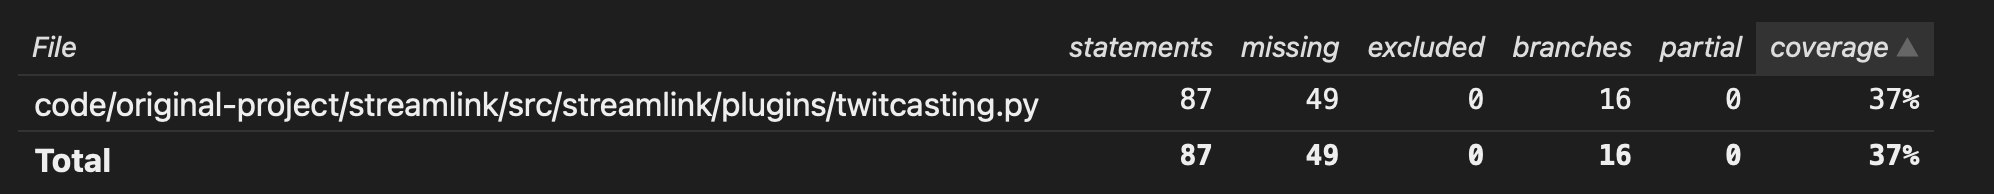
\includegraphics[width=0.8\textwidth]{twitcasting.png}
  \caption{Coverage of \texttt{twitcasting.py} Before Testing by Maxim Zilke}
  \label{fig:meinbild}
\end{figure}

[Yossef AL Buni]:\\ For the method \verb|M3U8Parser.parse_line|, I measured the test coverage using \verb|pytest| with the \verb|pytest-cov| plugin.The goal was to evaluate how thoroughly the existing test suite exercises this method with respect to both branch and line coverage.
\begin{itemize}
  \item \textbf{Line Coverage}: 86\%
  \item \textbf{Branch Coverage}: 8 branches in total, 2 of them only partially covered
  \item \textbf{Total Statements}: 13
  \item \textbf{Uncovered Statements}: 1
\end{itemize}
These coverage values indicate that the current test suite exercises the majority of the control flow paths through the method. However, two of the eight branches are only partially tested. This suggests that not all combinations of the conditions---particularly the three-clause predicate inside the first \texttt{if} statement---are fully covered by the tests.
A screenshot of the coverage report is attached below.
\begin{figure}[H]
  \centering
  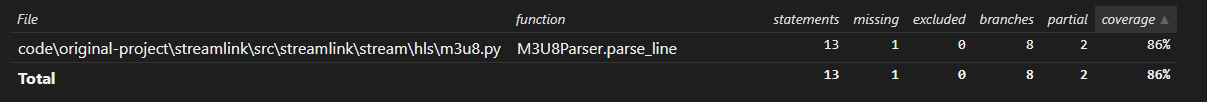
\includegraphics[width=0.8\textwidth]{parse_line.png}
  \caption{Function-Level Coverage Report: Coverage of \texttt{m3u8.parse\_line.py} Before Testing by Yossef Al Buni}
  \label{fig:yossefs_bild}
\end{figure}
\begin{figure}[H]
  \centering
  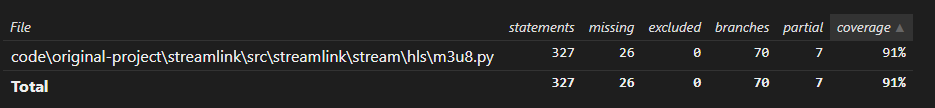
\includegraphics[width=0.8\textwidth]{m3u8.png}
  \caption{File-Level Coverage Report: Coverage of \texttt{m3u8.py} Before Testing by Yossef Al Buni}
  \label{fig:yossefs_bild}
\end{figure}

            % Include your screenshot of coverage report
            % \begin{figure}[h]
            %   \centering
            %   \includegraphics[width=0.8\textwidth]{your_screenshot_filename.jpg}
            %   \caption{Screenshot of Coverage Report}
            %   \label{fig:coverage}
            % \end{figure}
          \end{answer}

    \item Create a set of tests that satisfy \textit{three} of the following logic criteria (pick one concrete criterion from each of your three selected bullet points):
          \begin{itemize}
            \item \textit{Predicate Coverage} (PC), \textit{Clause Coverage} (CC), \textit{Combinatorial Coverage} (CoC)
            \item \textit{Active Clause Coverage} (ACC), \textit{General Active Clause Coverage} (GACC), \textit{Restricted Active Clause Coverage} (RACC), \textit{Correlated Active Clause Coverage} (CACC)
            \item \textit{Inactive Clause Coverage} (ICC), \textit{General Inactive Clause Coverage} (GICC), \textit{Restricted Inactive Clause Coverage} (RICC)
            \item \textit{Implicant Coverage} (IC)
            \item \textit{Multiple Unique True Point Coverage} (MUTP), \textit{Unique True Point and Near False Point Pair Coverage} (CUTPNFP), \textit{Multiple Near False Point Coverage} (MNFP)
          \end{itemize}
          \begin{answer}
\section*{ACC-Tests für \texttt{\_get\_streams() by Maxim Zilke}}
\lstset{
  language=Python,
  basicstyle=\ttfamily\small,
  keywordstyle=\color{blue},
  commentstyle=\color{gray},
  stringstyle=\color{orange},
  showstringspaces=false,
  breaklines=true,
  frame=single,
  numbers=left,
  numberstyle=\tiny,
  xleftmargin=2em,
  framexleftmargin=1.5em
}
\begin{lstlisting}[language=Python]
import hashlib
from streamlink import Streamlink
from streamlink.plugins.twitcasting import TwitCasting
from unittest.mock import MagicMock



def make_plugin(password=None):
    session = Streamlink()
    plugin = TwitCasting(session, "https://twitcasting.tv/testuser")
    plugin.match = {"channel": "testuser"}
    plugin.options = {"password": password} if password else {}
    return plugin



def test_acc_first_predicate_first_clause_true():
    plugin = make_plugin()
    plugin._api_query_streamserver = MagicMock(return_value=(
        None, {}, {}
    ))
    assert list(plugin._get_streams()) == []



def test_acc_first_predicate_first_clause_false():
    plugin = make_plugin()
    plugin._api_query_streamserver = MagicMock(return_value=(
        {"id": 123, "live": True}, {"streams": {"mytest": "https://twitcasting.tv/testuser"}}, None
    ))
    plugin._get_streams_websocket = MagicMock(return_value=iter(["ws_mytest", "https://twitcasting.tv/testuser"]))
    assert list(plugin._get_streams()) == ["ws_mytest", "https://twitcasting.tv/testuser"]




def test_acc_first_predicate_second_clause_true():
    plugin = make_plugin()
    plugin._api_query_streamserver = MagicMock(return_value=(
        {"id": None, "live": True}, {}, {}
    ))
    assert list(plugin._get_streams()) == []



def test_acc_first_predicate_second_clause_false():
    plugin = make_plugin()
    plugin._api_query_streamserver = MagicMock(return_value=(
        {"id": 123, "live": True}, {"streams": {"mytest": "https://twitcasting.tv/testuser"}}, None
    ))
    plugin._get_streams_websocket = MagicMock(return_value=iter(["ws_mytest", "https://twitcasting.tv/testuser"]))
    assert list(plugin._get_streams()) == ["ws_mytest", "https://twitcasting.tv/testuser"]



def test_acc_first_predicate_third_clause_true():
    plugin = make_plugin()
    plugin._api_query_streamserver = MagicMock(return_value=(
        {"id": 123, "live": False}, {}, {}
    ))
    assert list(plugin._get_streams()) == []



def test_acc_first_predicate_third_clause_false():
    plugin = make_plugin()
    plugin._api_query_streamserver = MagicMock(return_value=(
        {"id": 123, "live": True}, {"streams": {"mytest": "https://twitcasting.tv/testuser"}}, None
    ))
    plugin._get_streams_websocket = MagicMock(return_value=iter(["ws_mytest", "https://twitcasting.tv/testuser"]))
    assert list(plugin._get_streams()) == ["ws_mytest", "https://twitcasting.tv/testuser"]


def test_acc_second_predicate_first_clause_true():
    plugin = make_plugin()
    plugin._api_query_streamserver = MagicMock(return_value=(
        {"id": 1, "live": True}, None, None
    ))
    assert list(plugin._get_streams()) == []



def test_acc_second_predicate_first_clause_false():
    plugin = make_plugin()
    plugin._api_query_streamserver = MagicMock(return_value=(
        {"id": 1, "live": True}, {"streams": {"mytest": "https://twitcasting.tv/testuser"}}, None
    ))
    plugin._get_streams_websocket = MagicMock(return_value=iter(["ws_mytest", "https://twitcasting.tv/testuser"]))
    assert list(plugin._get_streams()) == ["ws_mytest", "https://twitcasting.tv/testuser"]




def test_acc_second_predicate_second_clause_true():
    plugin = make_plugin()
    plugin._api_query_streamserver = MagicMock(return_value=(
        {"id": 1, "live": True}, None, None  
    ))
    assert list(plugin._get_streams()) == []  




def test_acc_second_predicate_second_clause_false():
    plugin = make_plugin()
    plugin._api_query_streamserver = MagicMock(return_value=(
        {"id": 1, "live": True}, None, {"streams": {"mytest": "https://twitcasting.tv/testuser"}}
    ))
    plugin._get_streams_hls = MagicMock(return_value=iter(["hls_mytest"]))
    assert list(plugin._get_streams()) == ["hls_mytest"]


\end{lstlisting}
\section*{PC-Tests für \texttt{\_parse\_line() by Yossef Al Buni}}
\lstset{
  language=Python,
  basicstyle=\ttfamily\small,
  keywordstyle=\color{blue},
  commentstyle=\color{gray},
  stringstyle=\color{orange},
  showstringspaces=false,
  breaklines=true,
  frame=single,
  numbers=left,
  numberstyle=\tiny,
  xleftmargin=2em,
  framexleftmargin=1.5em
}
\begin{lstlisting}[language=Python]
# Covers: Predicate Coverage (PC) - Predicate is True
def test_parse_line_predicate_true():
    parser = M3U8Parser()
    line = "#"
    parser.split_tag = lambda l: ("", None)
    parser.parse_line(line)

# Covers: Predicate Coverage (PC) - Predicate is False
def test_parse_line_predicate_false():
    parser = M3U8Parser()
    line = "#EXTINF:10,"
    parser.split_tag = lambda l: ("EXTINF", "10")
    handler_mock = Mock()
    parser._TAGS = {"EXTINF": handler_mock}
    parser.parse_line(line)
    handler_mock.assert_called_once_with(parser, "10")
\end{lstlisting}
            

            % \begin{lstlisting}[style=pythongrey,belowskip=-0.8\baselineskip]
            % /* Add code here */
            % \end{lstlisting}
            % or: \lstinputlisting[language=Java,belowskip=-0.8\baselineskip]{file_name.java}
          \end{answer}

    \item Document for each individual test the coverage criterion / criteria it contributes to.
          \begin{answer}


     \begin{longtable}{|l|l|}
\caption{ACC Coverage Table for TwitCasting Tests by Maxim Zilke} \label{tab:acc-coverage} \\
\hline
\textbf{Test Case} & \textbf{Coverage Criterion} \\
\hline
\endfirsthead

\hline
\textbf{Test Case} & \textbf{Coverage Criterion} \\
\hline
\endhead

\hline
\multicolumn{2}{r}{\textit{Fortsetzung auf nächster Seite}} \\
\hline
\endfoot

\hline
\endlastfoot
%%%%%%%%%%%%%%%%%%%%%%%%%%%%%%%%%%%%%%%%%%%%%%%%%%%%%%%%%%%%%%%%%%%%%%%%%%%%%%%%
test\_acc\_first\_predicate\_first\_clause\_true & ACC (predicate 1, clause: movie) \\
test\_acc\_first\_predicate\_first\_clause\_false & ACC (predicate 1, clause: movie) \\
test\_acc\_first\_predicate\_second\_clause\_true & ACC (predicate 1, clause: id) \\
test\_acc\_first\_predicate\_second\_clause\_false & ACC (predicate 1, clause: id) \\
test\_acc\_first\_predicate\_third\_clause\_true & ACC (predicate 1, clause: live) \\
test\_acc\_first\_predicate\_third\_clause\_false & ACC (predicate 1, clause: live) \\
test\_acc\_second\_predicate\_first\_clause\_true & ACC (predicate 2, clause: websocket) \\
test\_acc\_second\_predicate\_first\_clause\_false & ACC (predicate 2, clause: websocket) \\
test\_acc\_second\_predicate\_second\_clause\_true & ACC (predicate 2, clause: hls) \\
test\_acc\_second\_predicate\_second\_clause\_false & ACC (predicate 2, clause: hls) \\
%%%%%%%%%%%%%%%%%%%%%%%%%%%%%%%%%%%%%%%%%%%%%%%%%%%%%%%%%%%%%%%%%%%%%%%%%%%%%%%%
test\_parse\_line\_predicate\_true & PC (predicate: line starts with "\#", condition is True) \\
test\_parse\_line\_predicate\_false & PC (predicate: line starts with "\#", condition is False) \\
%%%%%%%%%%%%%%%%%%%%%%%%%%%%%%%%%%%%%%%%%%%%%%%%%%%%%%%%%%%%%%%%%%%%%%%%%%%%%%%%

% other members

%%%%%%%%%%%%%%%%%%%%%%%%%%%%%%%%%%%%%%%%%%%%%%%%%%%%%%%%%%%%%%%%%%%%%%%%%%%%%%%%
\end{longtable}
          \end{answer}

%%%%%%%%%%%%%%%%%%%%%%%%%%%%%%%%%%%%%%%%%%%%%%%%%%%%%%%%%%%%%%%%%%%%%%%%%%%%%%%%
    \item Finally, recheck your method with the new, extended test suite regarding the \textit{branch} and \textit{line coverage} criteria, and explain \textit{how} their values have / have not changed.
          \begin{answer}
%%%%%%%%%%%%%%%%%%%%%%%%%%%%%%%%%%%%%%%%%%%%%%%%%%%%%%%%%%%%%%%%%%%%%%%%%%%%%%%%
After reviewing the test coverage of my project, I was able to increase the coverage of the \texttt{\_get\_streams()} function to \textbf{92\%}, up from an initial 0\%. Currently, one statement and one branch remain uncovered.

Full (100\%) coverage was not achieved because I did not include tests for \texttt{if} conditions consisting of a single clause. Such predicates are typically excluded from \textbf{Active Clause Coverage (ACC)} criteria.

Consequently, one single-clause \texttt{if} statement is not covered by the test suite. The other two \texttt{if} statements are covered in the analysis because they are indirectly triggered by existing test cases. [Maxim Zilke]

            \begin{figure}[h]
  \centering
  
\includegraphics[width=0.8\textwidth]{coverage_after_test.png}
  \caption{Coverage of \texttt{TwitCasting.\_get\_streams()} After Testing by Maxim Zilke}
  \label{fig:meinbild}
\end{figure}

%%%%%%%%%%%%%%%%%%%%%%%%%%%%%%%%%%%%%%%%%%%%%%%%%%%%%%%%%%%%%%%%%%%%%%%%%%%%%%%%

Yossef Al Buni: 
After adding the two new tests specifically targeting \textbf{Predicate Coverage (PC)} for the method \texttt{M3U8Parser.parse\_line}, we re-evaluated the instruction and branch coverage using \texttt{pytest} and the coverage plugin.
\begin{figure}[H]
\centering
\includegraphics[width=0.8\textwidth]{parse\_line\_after.png}
\caption{Function-Level Coverage Report: Coverage of \texttt{m3u8.parse\_line.py} After Testing by Yossef Al Buni}
\end{figure}
\begin{figure}[H]
\centering
\includegraphics[width=0.8\textwidth]{m3u8\_after.png}
\caption{File-Level Coverage Report: Coverage of \texttt{m3u8.py} After Testing by Yossef Al Buni}
\end{figure}
While the coverage percentages did not reach 100\%, the addition of the PC-focused test cases improved the granularity and intent of the test suite. The previously uncovered predicate paths in the condition
\begin{quote}
\texttt{if not tag or value is None or tag not in self.\_TAGS:}
\end{quote}
are now addressed more explicitly, and the test suite more thoroughly represents the logical structure of the method.
Although this did not eliminate the one remaining partially covered branch, the improvement from earlier measurements (86\% line coverage) to 95\% demonstrates a \textbf{measurable enhancement} in both branch and instruction testing quality. [Yossef Al Buni]
%%%%%%%%%%%%%%%%%%%%%%%%%%%%%%%%%%%%%%%%%%%%%%%%%%%%%%%%%%%%%%%%%%%%%%%%%%%%%%%%

% other members

%%%%%%%%%%%%%%%%%%%%%%%%%%%%%%%%%%%%%%%%%%%%%%%%%%%%%%%%%%%%%%%%%%%%%%%%%%%%%%%%
          \end{answer}
  \end{enumerate}
\end{question}

\begin{aiTask}
  Manually insert $2 * n$ faults into your selected methods. Follow the Differential-Prompting approach to generate failure-inducing tests. Evaluate the obtained tests by applying the 5 categories of test cases as specified in Section II of the paper.
  \begin{answer}
    [Group: Your Modifications]

    [Group: Differential-Prompting Steps]

    [Group: Your Results]

    \dots
    % \begin{lstlisting}[style=pythongrey]
    % [LLM tests]
    % \end{lstlisting}
    % or: \lstinputlisting[style=pythongrey]{file_name.py}
  \end{answer}
\end{aiTask}

\end{document}
